\documentclass[aspectratio=169]{beamer}

% The final-defense deck is intentionally based on the v1 proposal deck.
% Preserve its Madrid theme, typography, footer, and slide-layout vocabulary.
\usetheme{Madrid}
\usecolortheme{default}

\usepackage{amsmath}
\usepackage{amssymb}
\usepackage{amsthm}
\usepackage{graphicx}
\usepackage{tikz}
\usepackage{booktabs}
\usepackage{array}
\usepackage{natbib}
\usepackage{appendixnumberbeamer}

\bibliographystyle{plain}

% All displayed dissertation results resolve from v2/data/*.csv.
% macros.tex
% Late-binding citation macros for the dissertation paper.
%
% Every number in prose resolves at build time through these macros.
% Values are defined in generated/values.tex via \csname lookup;
% build_numbers.py produces that file from data/*.csv and
% generated/figures/*.numbers.csv.
%
% Namespace prefix: ds@ (dissertation). Must match NAMESPACE in build_numbers.py.
%
% Usage:
%   \result{csv_stem}{key}[precision]
%   \resdelta{csv_stem}{key_a}{key_b}[precision]
%   \resratio{csv_stem}{key_a}{key_b}[precision]
%   \resultCI{csv_stem}{mean_key,lo_key,hi_key}[precision]
%   \resultPM{csv_stem}{mean_key,err_key}[precision]
%
% Where:
%   csv_stem  - stem of the CSV file (e.g. "headline" for headline.csv,
%               "fig.02_signflip" for the sidecar of Figure 2 — note the
%               filename is still 02_signflip.* for build-pipeline stability
%               even though the §5.3 prose framing was retuned 2026-05-28;
%               see paper/05_results.md §5.3 for the rationale)
%   key       - colon-joined coordinate per the CSV's key_schema
%   precision - number of decimal places for siunitx rounding (optional;
%               default is the CSV's default_precision, embedded as
%               ds@<stem>@__default_precision__ in values.tex)

\usepackage{siunitx}
\usepackage{xfp}
\usepackage{etoolbox}

% --------------------------------------------------------------------------
% Definitions below use @ in macro names. Outside a .sty file, @ has catcode
% 12, so we temporarily make it a letter via \makeatletter / \makeatother.
% --------------------------------------------------------------------------
\makeatletter

% --------------------------------------------------------------------------
% Internal helper: look up \csname ds@<stem>@<key>\endcsname
% Raises \PackageError if undefined.
% --------------------------------------------------------------------------
\newcommand{\ocget}[2]{%
  \@ifundefined{ds@#1@#2}{%
    \PackageError{dissertation-macros}%
      {Undefined result key '#2' in CSV stem '#1'.
       Check data/#1.csv and re-run 'make values'.}%
      {The key '#2' was not found in the values generated from '#1'.
       Valid keys are listed in generated/values.tex.}%
    \textbf{??}%
  }{%
    \csname ds@#1@#2\endcsname%
  }%
}

% --------------------------------------------------------------------------
% Helper: get default precision for a CSV stem (falls back to 3)
% --------------------------------------------------------------------------
\newcommand{\ocgetdefprec}[1]{%
  \@ifundefined{ds@#1@__default_precision__}{3}{\csname ds@#1@__default_precision__\endcsname}%
}

% --------------------------------------------------------------------------
% \result{csv}{key}[precision]
% --------------------------------------------------------------------------
\DeclareRobustCommand{\result}[2]{%
  \@ifnextchar[%]
    {\ds@result@prec{#1}{#2}}%
    {\ds@result@prec{#1}{#2}[\ocgetdefprec{#1}]}%
}
\def\ds@result@prec#1#2[#3]{%
  \num[round-mode=places,round-precision=#3]{\ocget{#1}{#2}}%
}

% --------------------------------------------------------------------------
% \resdollar{csv}{key}[precision]
% Render a USD value with the sign OUTSIDE the dollar sign: a negative
% value prints as "-\$0.023", not "\$-0.023". Rounds first so that values
% that round to zero print "\$0.000" rather than "-\$0.000". Use inside
% math mode (the bare "-" is a math minus), mirroring the old
% "$\$\result{...}$" idiom that placed the minus after the dollar sign.
% --------------------------------------------------------------------------
\DeclareRobustCommand{\resdollar}[2]{%
  \@ifnextchar[%]
    {\ds@dollar@prec{#1}{#2}}%
    {\ds@dollar@prec{#1}{#2}[\ocgetdefprec{#1}]}%
}
\def\ds@dollar@prec#1#2[#3]{%
  \edef\ds@dv{\fpeval{round(\ocget{#1}{#2},#3)}}%
  \ifnum\fpeval{\ds@dv<0}=1 %
    -\$\num[round-mode=places,round-precision=#3]{\fpeval{abs(\ds@dv)}}%
  \else
    \$\num[round-mode=places,round-precision=#3]{\ds@dv}%
  \fi
}

% --------------------------------------------------------------------------
% \resdelta{csv}{key_a}{key_b}[precision]
% Computes key_a - key_b using \fpeval from xfp.
% (Named \resdelta, not \delta, to avoid clashing with the Greek letter.)
% --------------------------------------------------------------------------
\DeclareRobustCommand{\resdelta}[3]{%
  \@ifnextchar[%]
    {\ds@delta@prec{#1}{#2}{#3}}%
    {\ds@delta@prec{#1}{#2}{#3}[\ocgetdefprec{#1}]}%
}
\def\ds@delta@prec#1#2#3[#4]{%
  \edef\ds@va{\ocget{#1}{#2}}%
  \edef\ds@vb{\ocget{#1}{#3}}%
  \num[round-mode=places,round-precision=#4,explicit-sign]{\fpeval{\ds@va - \ds@vb}}%
}

% --------------------------------------------------------------------------
% \resratio{csv}{key_a}{key_b}[precision]
% Computes key_a / key_b using \fpeval.
% --------------------------------------------------------------------------
\DeclareRobustCommand{\resratio}[3]{%
  \@ifnextchar[%]
    {\ds@ratio@prec{#1}{#2}{#3}}%
    {\ds@ratio@prec{#1}{#2}{#3}[\ocgetdefprec{#1}]}%
}
\def\ds@ratio@prec#1#2#3[#4]{%
  \edef\ds@va{\ocget{#1}{#2}}%
  \edef\ds@vb{\ocget{#1}{#3}}%
  \num[round-mode=places,round-precision=#4]{\fpeval{\ds@va / \ds@vb}}%
}

% --------------------------------------------------------------------------
% \resp{csv}{key}[sigfigs]
% Render a p-value at N significant figures (default 2). Uses siunitx
% scientific notation automatically for small p (e.g. 2.7e-17 → 2.7×10⁻¹⁷),
% which `\result`'s round-mode=places would clobber to 0.000.
% --------------------------------------------------------------------------
\DeclareRobustCommand{\resp}[2]{%
  \@ifnextchar[%]
    {\ds@resp@prec{#1}{#2}}%
    {\ds@resp@prec{#1}{#2}[2]}%
}
\def\ds@resp@prec#1#2[#3]{%
  \num[round-mode=figures,round-precision=#3]{\ocget{#1}{#2}}%
}

% --------------------------------------------------------------------------
% \respp{csv}{key}[precision]
% Render a stored 0–1 fraction as percentage points: value × 100. Pass-rate
% deltas in paired_contrasts.csv are fractions; tables typically want pp.
% Default precision: 2 decimal places.
% --------------------------------------------------------------------------
\DeclareRobustCommand{\respp}[2]{%
  \@ifnextchar[%]
    {\ds@respp@prec{#1}{#2}}%
    {\ds@respp@prec{#1}{#2}[2]}%
}
\def\ds@respp@prec#1#2[#3]{%
  \num[round-mode=places,round-precision=#3]{\fpeval{100*\ocget{#1}{#2}}}%
}

% --------------------------------------------------------------------------
% \respct{csv}{delta_key}{ref_key}[precision]
% Render a paired-contrast delta as a percentage of a reference mean:
% (delta / ref) × 100, with a literal '%' appended. For "code-only is X%
% cheaper than competitor" framing, pass the contrast's mean_b cell as ref.
% Default precision: 1 decimal place.
% --------------------------------------------------------------------------
\DeclareRobustCommand{\respct}[3]{%
  \@ifnextchar[%]
    {\ds@respct@prec{#1}{#2}{#3}}%
    {\ds@respct@prec{#1}{#2}{#3}[1]}%
}
\def\ds@respct@prec#1#2#3[#4]{%
  \edef\ds@vd{\ocget{#1}{#2}}%
  \edef\ds@vr{\ocget{#1}{#3}}%
  \num[round-mode=places,round-precision=#4]{\fpeval{100*\ds@vd/\ds@vr}}\%%
}

% --------------------------------------------------------------------------
% \resultCI{csv}{mean_key,lo_key,hi_key}[precision]
% Renders as: mean [lo, hi]
% --------------------------------------------------------------------------
\DeclareRobustCommand{\resultCI}[2]{%
  \@ifnextchar[%]
    {\ds@ci@prec{#1}{#2}}%
    {\ds@ci@prec{#1}{#2}[\ocgetdefprec{#1}]}%
}
\def\ds@ci@prec#1#2[#3]{%
  \ds@splitthree{#2}{\ds@keyA}{\ds@keyB}{\ds@keyC}%
  \num[round-mode=places,round-precision=#3]{\ocget{#1}{\ds@keyA}}%
  \ [\num[round-mode=places,round-precision=#3]{\ocget{#1}{\ds@keyB}},
     \num[round-mode=places,round-precision=#3]{\ocget{#1}{\ds@keyC}}]%
}

% --------------------------------------------------------------------------
% \resultPM{csv}{mean_key,err_key}[precision]
% Renders as: mean ± err
% --------------------------------------------------------------------------
\DeclareRobustCommand{\resultPM}[2]{%
  \@ifnextchar[%]
    {\ds@pm@prec{#1}{#2}}%
    {\ds@pm@prec{#1}{#2}[\ocgetdefprec{#1}]}%
}
\def\ds@pm@prec#1#2[#3]{%
  \ds@splittwo{#2}{\ds@keyA}{\ds@keyB}%
  \num[round-mode=places,round-precision=#3]{\ocget{#1}{\ds@keyA}}%
  $\pm$%
  \num[round-mode=places,round-precision=#3]{\ocget{#1}{\ds@keyB}}%
}

% --------------------------------------------------------------------------
% Utility: split comma-delimited pairs and triples into named macros.
% --------------------------------------------------------------------------
\def\ds@splittwo#1#2#3{%
  \ds@splittwoaux#1\@nil{#2}{#3}%
}
\def\ds@splittwoaux#1,#2\@nil#3#4{%
  \def#3{#1}\def#4{#2}%
}

\def\ds@splitthree#1#2#3#4{%
  \ds@splitthreeaux#1\@nil{#2}{#3}{#4}%
}
\def\ds@splitthreeaux#1,#2,#3\@nil#4#5#6{%
  \def#4{#1}\def#5{#2}\def#6{#3}%
}

\makeatother

\input{generated/values.tex}

\graphicspath{{figures/}{generated/figures/}{../v1/images/}}

\title[What Representations Preserve]{What Representations Preserve:\\Information-Theoretic and Geometric Conditions for\\Out-of-Distribution and Hallucination Detection}
\subtitle{PhD Dissertation Defense}
\author{Hong Yang}
\institute{Rochester Institute of Technology}
\date{August 7, 2026}

\setbeamertemplate{navigation symbols}{}

% The same two-part footer used by the proposal deck.
\newcommand{\sectionpubinfo}{}
\setbeamertemplate{footline}{
  \leavevmode%
  \hbox{%
  \begin{beamercolorbox}[wd=.5\paperwidth,ht=2.25ex,dp=1ex,left]{author in head/foot}%
    \usebeamerfont{author in head/foot}\hspace*{2ex}\insertsectionhead\sectionpubinfo
  \end{beamercolorbox}%
  \begin{beamercolorbox}[wd=.5\paperwidth,ht=2.25ex,dp=1ex,right]{title in head/foot}%
    \usebeamerfont{title in head/foot}\insertframenumber{} / \inserttotalframenumber\hspace*{2ex}
  \end{beamercolorbox}}%
  \vskip0pt%
}

\newcommand{\scopefooter}[1]{%
  \vfill
  \begin{center}
    \footnotesize\textbf{Scope:} #1
  \end{center}%
}

\begin{document}

% ---------------------------------------------------------------------------
% 1--4. Introduction
% ---------------------------------------------------------------------------

% 1
\begin{frame}
  \titlepage
\end{frame}

\section{Introduction}

% 2
\begin{frame}{Why confidence can be misleading}
\begin{itemize}
  \item \textbf{An unfamiliar input can still receive a confident prediction.}
  \begin{itemize}
    \item A system trained to read chest X-rays is shown a brain MRI.
    \item The system can still produce a confident diagnosis, even though the image is unlike its training examples.
  \end{itemize}
  \item \textbf{An unsupported answer can still sound convincing.}
  \begin{itemize}
    \item A language model produces a polished citation.
    \item The cited source does not exist, but the wording alone may not reveal that.
  \end{itemize}
  \item \textbf{The shared problem:} confidence tells us what the model chose, not whether it had the evidence needed to choose it.
\end{itemize}

\vfill
\begin{center}
  \large What must the model preserve internally for a detector to recognize these failures?
\end{center}
\end{frame}

% 3
\begin{frame}{Two lenses tell us what a detector can recover}
\begin{itemize}
  \item \textbf{A representation} is the internal description a model builds from its input.
  \begin{itemize}
    \item A detector sees this description or a score derived from it---not the information the model already discarded.
  \end{itemize}
  \item \textbf{Information theory asks whether the needed distinction remains.}
  \begin{align*}
    I(Z;Y)>0 \quad &\text{means that representation } Z \text{ retains some information about target } Y.
  \end{align*}
  \item \textbf{Representation geometry asks where the surviving variation lives.}
  \begin{itemize}
    \item Is it spread across useful directions, or compressed into a narrow class-focused subspace?
  \end{itemize}
\end{itemize}

\vfill
\begin{center}
  \textbf{Information theory tests presence; geometry tests accessibility.}
\end{center}
\end{frame}

% 4
\begin{frame}{Presentation Roadmap}
\begin{itemize}
  \item \textbf{Three completed studies}:
  \begin{enumerate}
    \item \textcolor{blue}{\textbf{Failure---Label Blindness:}} when unlabeled training removes the label distinction.
    \item \textcolor{green!60!black}{\textbf{Recovery---DSC and TGT:}} when supervised training suppresses domain sensitivity and guidance restores it.
    \item \textcolor{red}{\textbf{Detection---Hallucination probe:}} when a frozen language model retains a signal that a learned readout can expose.
  \end{enumerate}
  \item \textbf{Presentation structure}:
  \begin{itemize}
    \item High-level overview of all three contributions.
    \item Technical deep dive into the question, method, evidence, and limitations of each study.
    \item Synthesis into a representation-first decision rule.
  \end{itemize}
  \item \textbf{Unifying thesis}: detection succeeds only when the representation preserves the structure that distinguishes the failure.
\end{itemize}
\end{frame}

% ---------------------------------------------------------------------------
% 5--7. Research overview
% ---------------------------------------------------------------------------

\section{Research Overview}

% 5
\begin{frame}{Contribution 1: Label Blindness in Unlabeled OOD Detection}
\begin{itemize}
  \item \textbf{Question}: Can a representation learned without class labels preserve the distinctions needed for class-based OOD detection?
  \item \textbf{Conditional failure result}:
  \begin{itemize}
    \item The input decomposes into independent feature components.
    \item The surrogate task depends on one component; the ID/OOD label depends on the other.
    \item A minimal sufficient representation for the surrogate contains no information about the ID/OOD label.
  \end{itemize}
  \item \textbf{Evaluation contribution}: Adjacent OOD holds out classes from the same dataset, removing easy domain shortcuts.
  \item \textbf{Evidence}: unlabeled methods move toward chance on Faces, Cars, and Food while supervised MSP remains substantially stronger.
\end{itemize}
\scopefooter{This is a theorem under explicit independence and minimal-sufficiency assumptions, not a claim that all self-supervision fails.}
\end{frame}

% 6
\begin{frame}{Contribution 2: Domain-Sensitivity Collapse and Recovery}
\begin{itemize}
  \item \textbf{Problem}: single-domain labels reward class separation but do not reward sensitivity to acquisition domain, modality, or style.
  \item \textbf{Diagnosis---Domain-Sensitivity Collapse (DSC)}:
  \begin{itemize}
    \item Cross-entropy features become highly anisotropic and concentrate near a low-rank class subspace.
    \item Domain-shift directions survive only in low-variance tails, weakening both distance- and logit-based scores.
  \end{itemize}
  \item \textbf{Recovery---Teacher-Guided Training (TGT)}:
  \begin{itemize}
    \item Distill the class-suppressed residual of a frozen multi-domain teacher during training.
    \item Discard the teacher and auxiliary head at inference.
  \end{itemize}
  \item \textbf{Evidence}: restored effective rank tracks lower FPR@95 across the evaluated scorers.
\end{itemize}
\scopefooter{DSC provides diagnostic bounds and testable predictions; it is not an impossibility theorem.}
\end{frame}

% 7
\begin{frame}{Contribution 3: Cross-Layer Hallucination Detection}
\begin{itemize}
  \item \textbf{Question}: Does a frozen language model's residual stream retain a signal that separates truthful from incorrect short answers?
  \item \textbf{Method}:
  \begin{itemize}
    \item Treat two intermediate layers from one forward pass as paired views.
    \item Learn a shared compressor with asymmetric one-class contrastive supervision and log-probability reconstruction.
    \item Score distance from a bank of truthful training examples.
  \end{itemize}
  \item \textbf{Evidence}:
  \begin{itemize}
    \item The principled probe reaches parity with the strongest engineered activation probe.
    \item A theory-predicted failure of symmetric supervision appears in the ablation.
  \end{itemize}
  \item \textbf{Access regime}: two open-weight 8B models, white-box activations, one forward pass.
\end{itemize}
\scopefooter{The contribution is a principled and self-validating readout, not a universal or state-of-the-art claim.}
\end{frame}

% ---------------------------------------------------------------------------
% 8--14. Label Blindness deep dive
% ---------------------------------------------------------------------------

\renewcommand{\sectionpubinfo}{\hspace{1ex}(Chapter 4 --- ICLR 2025)}
\section{Label Blindness Deep Dive}

% 8
\begin{frame}{Motivating Example: When Features Mislead}
\begin{center}
  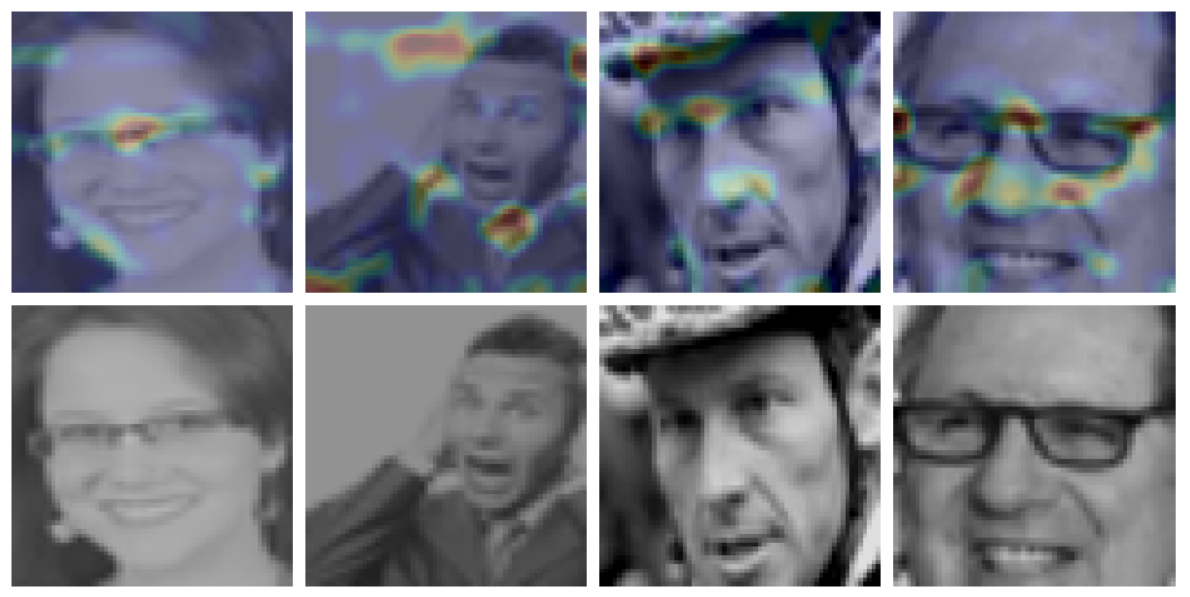
\includegraphics[width=0.68\textwidth]{gradcam_example_faces.png}
\end{center}
\vspace{0.1cm}
\small\textbf{An unlabeled representation may emphasize easy visual regularities, such as glasses, rather than the facial-expression distinction used by the downstream label.}

\vspace{0.1cm}
\footnotesize GradCAM is diagnostic evidence, not proof of feature independence~\citep{selvaraju2017grad}.
\end{frame}

% 9
\begin{frame}{Formal Problem Definition}
\begin{itemize}
  \item \textbf{OOD detection task}:
  \begin{itemize}
    \item Training examples come from an in-distribution label set $\mathcal{Y}_{\mathrm{ID}}$.
    \item At test time, the detector must distinguish those examples from held-out labels $\mathcal{Y}_{\mathrm{OOD}}$.
  \end{itemize}
  \item \textbf{Two training signals}:
  \begin{itemize}
    \item The surrogate target $Y_s=f_1(X_1)$ is available without class labels.
    \item The desired ID/OOD distinction $Y=f_2(X_2)$ depends on a different feature component.
  \end{itemize}
  \item \textbf{Label-blind setting}:
  \begin{align*}
    X=(X_1,X_2),\qquad X_1\perp X_2,
  \end{align*}
  and $Z$ is a minimal sufficient representation for $Y_s$.
  \item \textbf{Research question}: What can any detector restricted to $Z$ recover about $Y$?
\end{itemize}
\end{frame}

% 10
\begin{frame}{Information-Theoretic Analysis}
\begin{itemize}
  \item \textbf{Minimality removes information unused by the surrogate task.}
  \begin{align*}
    Y_s=f_1(X_1),\quad X_1\perp X_2
    \quad\Longrightarrow\quad I(X_2;Z)=0.
  \end{align*}
  \item \textbf{The ID/OOD label depends only on the discarded component.}
  \begin{align*}
    Y=f_2(X_2)
    \quad\Longrightarrow\quad I(Y;Z)=0.
  \end{align*}
  \item \textbf{Consequence}: every statistic computed only from $Z$ is blind to the missing label distinction.
  \item \textbf{Why filtering does not help}: selecting ID classes from the population does not create dependence between the originally independent feature components.
\end{itemize}
\scopefooter{The strict result requires the stated independence and minimal-sufficiency conditions. Approximate dependence yields a warning, not the same guarantee.}
\end{frame}

% 11
\begin{frame}{Adjacent OOD Evaluation Paradigm}
\begin{itemize}
  \item \textbf{Far OOD can be solved using broad domain differences.}
  \begin{itemize}
    \item Example: CIFAR-10 versus MNIST.
  \end{itemize}
  \item \textbf{Near OOD reduces those differences but often changes the source dataset.}
  \begin{itemize}
    \item Example: CIFAR-10 versus CIFAR-100.
  \end{itemize}
  \item \textbf{Adjacent OOD uses one dataset and holds out classes.}
  \begin{itemize}
    \item Faces, Cars, and Food share acquisition style, background statistics, and visual nuisance factors.
    \item Only the semantic class distinction reliably separates ID from OOD.
  \end{itemize}
  \item \textbf{Evaluation}: three random class splits; report AUROC and FPR@95.
\end{itemize}

\vfill
\begin{center}
  \textbf{High feature overlap turns label dependence into the intended stress test.}
\end{center}
\end{frame}

% 12
\begin{frame}{Empirical Validation Results}
\begin{center}
  \includegraphics[height=0.68\textheight]{defense_label_blindness_auroc.pdf}
\end{center}
\vspace{-0.1cm}
\begin{center}
  \small Unlabeled methods fall toward chance on the high-overlap task; supervised MSP preserves a clear advantage.
\end{center}
\end{frame}

% 13
\begin{frame}{What the Label Blindness Result Establishes}
\begin{columns}[T]
\begin{column}{0.48\textwidth}
\begin{block}{Established}
\begin{itemize}
  \item Strict independence gives a genuine no-signal result.
  \item Adjacent OOD targets cases where the label distinction matters.
  \item A better post-hoc score cannot reconstruct information absent from $Z$.
\end{itemize}
\end{block}
\end{column}
\begin{column}{0.48\textwidth}
\begin{alertblock}{Not established}
\begin{itemize}
  \item Every self-supervised objective is label blind.
  \item High image overlap proves statistical independence.
  \item A detector with labels, external data, or another representation must fail.
\end{itemize}
\end{alertblock}
\end{column}
\end{columns}

\vfill
\begin{center}
  \textbf{The theorem identifies a boundary condition and the benchmark makes that boundary visible.}
\end{center}
\end{frame}

% 14
\begin{frame}{Label Blindness: Key Takeaways}
\begin{itemize}
  \item \textbf{Theoretical contribution}:
  \begin{itemize}
    \item Formalizes when a minimal surrogate representation contains no information about the desired OOD label.
    \item Connects representation sufficiency to a downstream detection limit.
  \end{itemize}
  \item \textbf{Methodological contribution}:
  \begin{itemize}
    \item Adjacent OOD removes domain shortcuts and tests the label-dependent distinction directly.
    \item Faces, Cars, and Food expose the predicted weakness across several unlabeled method families.
  \end{itemize}
  \item \textbf{Practical implication}:
  \begin{itemize}
    \item Before changing the OOD score, ask whether the training objective preserved the needed distinction.
  \end{itemize}
  \item \textbf{Status}: published at ICLR 2025.
\end{itemize}
\end{frame}

% ---------------------------------------------------------------------------
% 15--22. DSC and TGT deep dive
% ---------------------------------------------------------------------------

\renewcommand{\sectionpubinfo}{\hspace{1ex}(Chapter 5 --- Under review, 2026)}
\section{DSC and TGT Deep Dive}

% 15
\begin{frame}{Motivating Question: What Do We Really Learn?}
\begin{columns}
\begin{column}{0.5\textwidth}
  \centering
  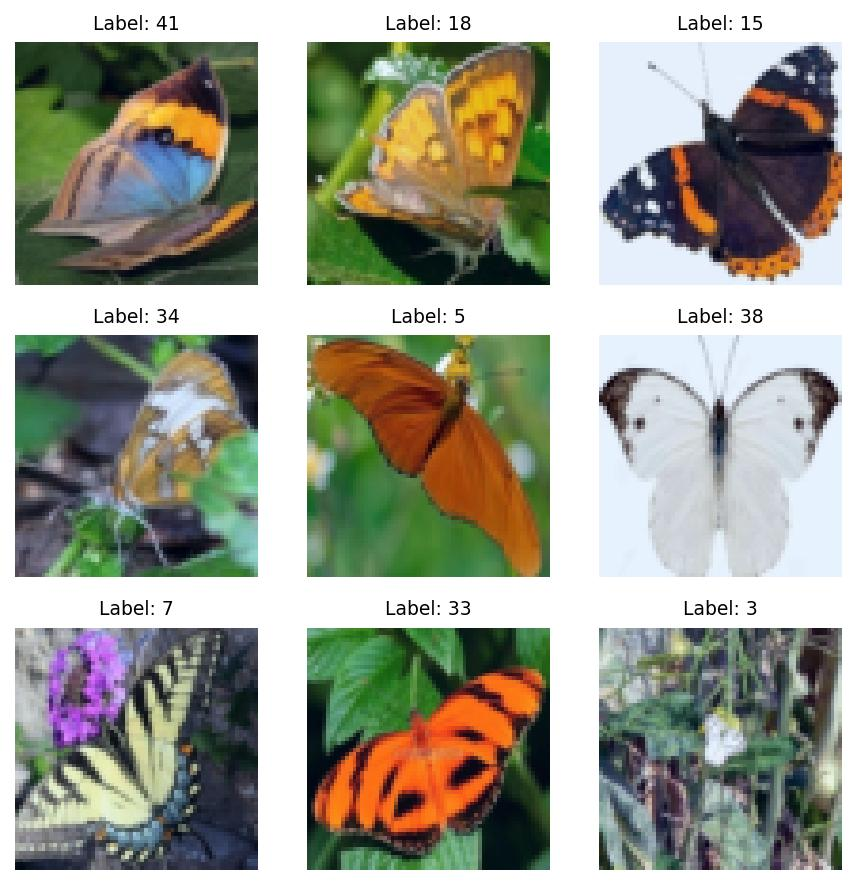
\includegraphics[width=0.9\textwidth]{butterfly_1_sample.jpg}
\end{column}
\begin{column}{0.5\textwidth}
  \centering
  \vspace{0.8cm}
  \Large
  \textbf{A classifier learns to separate butterfly species.}\\[0.65cm]
  \textbf{Does it remain sensitive to shape, sensor, texture, and acquisition domain?}
\end{column}
\end{columns}
\end{frame}

% 16
\begin{frame}{Mathematical Formalization}
\begin{itemize}
  \item \textbf{Single-domain supervised learning}: labels reward separation among $C$ known classes inside one visual domain.
  \item \textbf{Feature covariance separates two sources of variation}:
  \begin{align*}
    \Sigma=\Sigma_{\mathrm{between}}+\Sigma_{\mathrm{within}}.
  \end{align*}
  \item \textbf{Domain-Sensitivity Collapse (DSC)}:
  \begin{itemize}
    \item Within-class variance shrinks during cross-entropy training.
    \item Most energy concentrates near the $(C-1)$-dimensional class subspace.
    \item Directions that distinguish domain shift are pushed into a low-variance tail.
  \end{itemize}
  \item \textbf{Measured signature}: low effective rank
  \begin{align*}
    r_{\mathrm{eff}}(\Sigma)=\exp\!\left(-\sum_i p_i\log p_i\right),
    \qquad p_i=\frac{\lambda_i}{\sum_j\lambda_j}.
  \end{align*}
\end{itemize}
\end{frame}

% 17
\begin{frame}{Theoretical Analysis of Collapse}
\small
\begin{itemize}
  \item \textbf{Variance--discriminability mismatch}: the ID/OOD shift can live in directions whose ID variance is too small for ordinary distance scores to emphasize.
  \begin{align*}
    W_1\!\left(S_{\mathrm{KNN}}(Z_{\mathrm{ID}}),S_{\mathrm{KNN}}(Z_{\mathrm{OOD}})\right)
    \le L_k\varepsilon+4L_k\tau^2.
  \end{align*}
  \item \textbf{Head insensitivity}: if the classifier head aligns with the dominant class subspace, MSP and Energy inherit the same suppressed tail.
  \begin{align*}
    W_1\!\left(S(\ell_{\mathrm{ID}}),S(\ell_{\mathrm{OOD}})\right)
    \le \lVert W\rVert_{\mathrm{op}}\varepsilon+L_S\eta\tau.
  \end{align*}
  \item \textbf{Prediction}: low tail energy and low effective rank should coincide with weak OOD-score separation.
\end{itemize}
\scopefooter{These are diagnostic upper bounds under measurable DSC conditions; outside that regime they may be loose or vacuous.}
\end{frame}

% 18
\begin{frame}{Empirical Demonstration of DSC}
\begin{center}
  \includegraphics[height=0.69\textheight]{defense_dsc_geometry.pdf}
\end{center}
\vspace{-0.1cm}
\begin{center}
  \small Cross-entropy features are severely anisotropic on homogeneous datasets; teacher-guided training usually restores rank.
\end{center}
\end{frame}

% 19
\begin{frame}{Teacher-Guided Training Methodology}
\begin{itemize}
  \item \textbf{Teacher signal}: extract features from a frozen DINOv2 model trained across many visual domains.
  \item \textbf{Remove the teacher's class direction}:
  \begin{itemize}
    \item Project out the teacher subspace most aligned with the current dataset's class labels.
    \item The remaining residual emphasizes domain, style, texture, and other complementary structure.
  \end{itemize}
  \item \textbf{Guide the student during ordinary supervised training}:
  \begin{align*}
    \mathcal{L}_{\mathrm{TGT}}
      =\mathcal{L}_{\mathrm{CE}}
      +\lambda_{\mathrm{TGT}}\,
       \mathbb{E}_x\!\left[1-\cos\!\left(\hat h(Z),\hat u_{\mathrm{dom}}(x)\right)\right].
  \end{align*}
  \item \textbf{Inference}: discard the frozen teacher and auxiliary domain head; apply any post-hoc OOD score to the student features.
\end{itemize}

\vfill
\begin{center}
  \textbf{TGT changes training, not the test-time detector.}
\end{center}
\end{frame}

% 20
\begin{frame}{Implementation and Validation}
\begin{center}
  \includegraphics[height=0.69\textheight]{defense_dsc_fpr95.pdf}
\end{center}
\vspace{-0.1cm}
\begin{center}
  \small TGT improves all eight scorers on average; the largest and most consistent reductions occur for the distance-based methods predicted by DSC.
\end{center}
\end{frame}

% 21
\begin{frame}{Recovered Geometry Tracks Lower OOD Error}
\begin{center}
  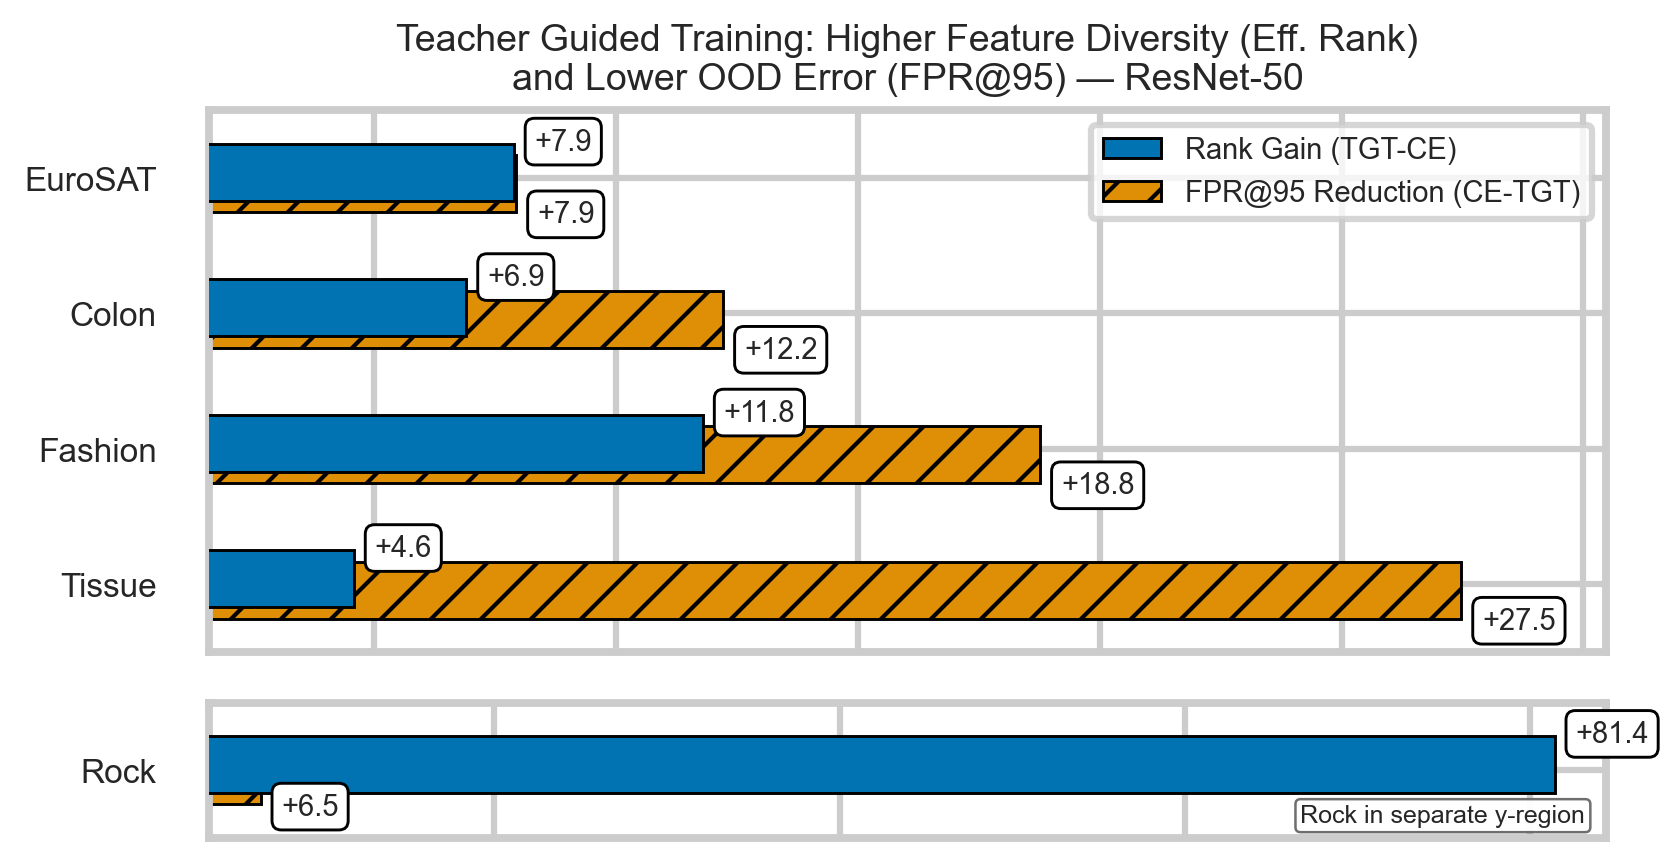
\includegraphics[height=0.70\textheight]{dsc_rank_vs_fpr95_gains.png}
\end{center}
\vspace{-0.1cm}
\begin{center}
  \small Across datasets, the increase in effective rank moves with the reduction in FPR@95---the proposed mechanism changes with the outcome.
\end{center}
\end{frame}

% 22
\begin{frame}{DSC and TGT: Key Takeaways}
\begin{itemize}
  \item \textbf{Diagnostic contribution}:
  \begin{itemize}
    \item DSC connects feature anisotropy and suppressed domain directions to the failure of distance- and logit-based OOD scores.
    \item The theory makes testable geometric predictions rather than a universal impossibility claim.
  \end{itemize}
  \item \textbf{Method contribution}:
  \begin{itemize}
    \item TGT transfers a class-suppressed teacher residual during training and adds no inference overhead.
    \item Mean effective rank rises from \result{dsc_geometry}{mean:ce:r_eff} to \result{dsc_geometry}{mean:tgt:r_eff} across the eight benchmarks.
  \end{itemize}
  \item \textbf{Limitations}:
  \begin{itemize}
    \item Gains vary by scorer and teacher--student pairing.
    \item Same-domain held-out classes remain difficult; TGT improves but does not solve that regime.
  \end{itemize}
  \item \textbf{Status}: under review, 2026.
\end{itemize}
\end{frame}

% ---------------------------------------------------------------------------
% 23--31. Hallucination detection deep dive
% ---------------------------------------------------------------------------

\renewcommand{\sectionpubinfo}{\hspace{1ex}(Chapter 6 --- In preparation, 2026)}
\section{Hallucination Detection Deep Dive}

% 23
\begin{frame}{Information-Theoretic Hallucination Framework}
\begin{itemize}
  \item \textbf{Access regime}: a frozen language model generates an answer while the detector reads its intermediate residual-stream activations.
  \item \textbf{Why cross-layer views are feasible}:
  \begin{itemize}
    \item Later residual states are deterministic functions of earlier states and intervening blocks.
    \item Consequently, different layers from the same forward pass share information.
  \end{itemize}
  \item \textbf{Trainability test}:
  \begin{align*}
    I(Z_a;Z_b)\ge \log K-\mathcal{L}_{\mathrm{InfoNCE}}.
  \end{align*}
  If the views were independent, the loss could not descend below the no-information floor $\log K$.
  \item \textbf{Empirical burden}: detection performance must still show that the shared information contains a label-relevant slice.
\end{itemize}
\scopefooter{Positive cross-layer dependence alone does not prove that hallucination labels are recoverable.}
\end{frame}

% 24
\begin{frame}{One-Class Contrastive Learning over Layer Pairs}
\begin{itemize}
  \item \textbf{Views}: two different layers from the same unaugmented generation, compressed by one shared network $f_\theta$.
  \item \textbf{Truthful examples form the coherent reference class}:
  \begin{itemize}
    \item Other truthful examples and the anchor's other-layer view are positives.
  \end{itemize}
  \item \textbf{Hallucinated examples are not forced into one cluster}:
  \begin{itemize}
    \item Only the example's own other-layer view is positive; other hallucinations remain negatives.
  \end{itemize}
  \item \textbf{Training objective}:
  \begin{align*}
    \mathcal{L}=\mathcal{L}_{\mathrm{SupCon\text{-}asym}}
      +\lambda\mathcal{L}_{\mathrm{logprob\text{-}recon}}.
  \end{align*}
  \item \textbf{Prediction}: symmetric class supervision should degrade detection when hallucinations lack coherent shared structure.
\end{itemize}
\end{frame}

% 25
\begin{frame}{System Architecture Details}
\begin{itemize}
  \item \textbf{Activation extraction}:
  \begin{itemize}
    \item Cache full response-token activation sequences from a mid-to-late layer band.
    \item No extra generation, retrieval system, or external verifier is required.
  \end{itemize}
  \item \textbf{Shared progressive compressor}:
  \begin{itemize}
    \item Transformer blocks reduce $4096\rightarrow2048\rightarrow1024\rightarrow512$ dimensions.
    \item Mean pooling produces one embedding for each generation--layer view.
  \end{itemize}
  \item \textbf{Two supervision channels}:
  \begin{itemize}
    \item Asymmetric one-class contrastive separation.
    \item Per-token log-probability reconstruction.
  \end{itemize}
  \item \textbf{Detection}: KNN distance from the truthful training bank; the base language model remains frozen.
\end{itemize}
\end{frame}

% 26
\begin{frame}{Experimental Design and Datasets}
\begin{itemize}
  \item \textbf{Models}: Llama-3.1-8B-Instruct and Qwen3-8B.
  \item \textbf{Short-answer QA datasets}:
  \begin{itemize}
    \item HotpotQA, Natural Questions, PopQA, SciQ, and SearchQA.
  \end{itemize}
  \item \textbf{Comparator families}:
  \begin{itemize}
    \item Output-space scalars, including log-probability-based scores.
    \item Single-pass activation probes, including SAPLMA and ACT-ViT.
    \item $K=10$ sampling methods, including semantic entropy and SelfCheckGPT.
  \end{itemize}
  \item \textbf{Protocol}: train and evaluate within each model--dataset cell over five seeds; report AUROC.
  \item \textbf{Operational label}: an answer is a hallucination when the benchmark evaluator marks the short answer incorrect.
\end{itemize}
\end{frame}

% 27
\begin{frame}{Results and Performance Analysis}
\begin{center}
  \includegraphics[height=0.69\textheight]{hd_headline.pdf}
\end{center}
\vspace{-0.1cm}
\begin{center}
  \small The principled probe reaches parity with ACT-ViT: three clear wins, three ties, one mean loss inside variance, and three clear ACT-ViT wins.
\end{center}
\end{frame}

% 28
\begin{frame}{Single-Pass Activation Readers Beat Ten-Sample Methods}
\begin{center}
  \includegraphics[height=0.61\textheight]{hd_compute_matched.pdf}
\end{center}
\vspace{-0.1cm}
\begin{center}
  \small Activation readers use one forward pass and consistently outperform the $K=10$ sampling family.
\end{center}
\scopefooter{ACT-ViT shares the same one-pass advantage; this distinguishes activation access from sampling, not our probe from ACT-ViT.}
\end{frame}

% 29
\begin{frame}{Ablations Identify the Supervision That Matters}
\begin{columns}[T]
\begin{column}{0.70\textwidth}
  \centering
  \includegraphics[width=\linewidth]{defense_hallu_attribution.pdf}
\end{column}
\begin{column}{0.28\textwidth}
\begin{itemize}
  \item \textbf{Reconstruction alone} adds little.
  \item \textbf{One-class contrast} carries nearly all of the measured gain.
  \item \textbf{Symmetric supervision} substantially degrades both models, as predicted.
\end{itemize}
\end{column}
\end{columns}
\scopefooter{The exact symmetric-run magnitudes remain gated pending import of the final run CSV.}
\end{frame}

% 30
\begin{frame}{The Learned Signal Transfers across QA Datasets}
\begin{center}
  \includegraphics[height=0.61\textheight]{hd_transfer.pdf}
\end{center}
\vspace{-0.1cm}
\begin{center}
  \small Cross-dataset transfer remains competitive with ACT-ViT, suggesting that the probe is not only memorizing a dataset's surface form.
\end{center}
\scopefooter{Transfer is variable rather than universal; Natural Questions remains the weakest source.}
\end{frame}

% 31
\begin{frame}{Hallucination Detection: Key Takeaways}
\begin{itemize}
  \item \textbf{Feasibility contribution}:
  \begin{itemize}
    \item Cross-layer dependence makes a contrastive readout well posed.
    \item Loss descent and downstream detection show that a label-relevant slice survives compression.
  \end{itemize}
  \item \textbf{Method contribution}:
  \begin{itemize}
    \item Different layers of one forward pass act as paired views.
    \item One-class supervision avoids inventing a coherent hallucination cluster.
  \end{itemize}
  \item \textbf{Empirical conclusion}:
  \begin{itemize}
    \item The method reaches parity with the strongest engineered activation probe and confirms a predicted ablation failure.
  \end{itemize}
  \item \textbf{Limits}: white-box access, two open-weight 8B models, short-answer tasks, evaluator-defined labels, and weak Natural Questions results.
\end{itemize}
\end{frame}

% ---------------------------------------------------------------------------
% 32--36. Synthesis and conclusion
% ---------------------------------------------------------------------------

\renewcommand{\sectionpubinfo}{}
\section{Synthesis \& Conclusion}

% 32
\begin{frame}{The Three Studies Address Three States of the Signal}
\begin{itemize}
  \item \textcolor{blue}{\textbf{Absent---Label Blindness}}
  \begin{itemize}
    \item Under strict assumptions, the learned representation contains no information about the required label distinction.
    \item \textbf{Intervention}: change the objective, labels, inputs, or representation.
  \end{itemize}
  \item \textcolor{green!60!black}{\textbf{Suppressed---DSC and TGT}}
  \begin{itemize}
    \item Domain sensitivity survives only in low-variance directions that standard scores use poorly.
    \item \textbf{Intervention}: repair the representation during training.
  \end{itemize}
  \item \textcolor{red}{\textbf{Retained---Cross-layer hallucination signal}}
  \begin{itemize}
    \item Intermediate activations preserve a usable distinction that output-only scores can obscure.
    \item \textbf{Intervention}: learn an appropriate readout.
  \end{itemize}
\end{itemize}

\vfill
\begin{center}
  \Large \textbf{Failure $\longrightarrow$ recovery $\longrightarrow$ detection}
\end{center}
\end{frame}

% 33
\begin{frame}{The Contribution Types Have Different Claim Strengths}
\centering
\small
\renewcommand{\arraystretch}{1.3}
\begin{tabular}{>{\raggedright\arraybackslash}p{2.2cm}>{\raggedright\arraybackslash}p{3.3cm}>{\raggedright\arraybackslash}p{4.0cm}}
\toprule
\textbf{Study} & \textbf{Evidence} & \textbf{Defensible conclusion} \\
\midrule
\textcolor{blue}{\textbf{Label Blindness}} & Conditional theorem and Adjacent-OOD stress test & A genuine failure boundary under independence and minimal sufficiency \\
\textcolor{green!60!black}{\textbf{DSC and TGT}} & Diagnostic bounds, geometry measurements, and intervention & Suppressed sensitivity can be diagnosed and partially restored \\
\textcolor{red}{\textbf{Hallucination}} & Feasibility argument, parity result, and predicted ablation & Retained internal signal supports a principled learned readout \\
\bottomrule
\end{tabular}

\vfill
\begin{itemize}
  \item \textbf{Information theory} determines whether target dependence remains.
  \item \textbf{Representation geometry} determines how surviving variation is organized for the detector.
\end{itemize}
\end{frame}

% 34
\begin{frame}{Limitations Define the Next Experiments}
\begin{itemize}
  \item \textbf{Label Blindness}: strict independence is a boundary condition.
  \begin{itemize}
    \item Measure degrees of blindness and study representations that deliberately retain multiple task factors.
  \end{itemize}
  \item \textbf{DSC and TGT}: the formal link between geometry and information loss remains incomplete; TGT inherits teacher coverage.
  \begin{itemize}
    \item Derive linking conditions, compare complementary teachers, and target the difficult in-domain regime.
  \end{itemize}
  \item \textbf{Hallucination detection}: the evidence is white-box and limited to short-answer QA.
  \begin{itemize}
    \item Explain the Natural Questions failure, broaden models and tasks, and test whether the signal supports mitigation rather than detection alone.
  \end{itemize}
\end{itemize}

\vfill
\begin{center}
  \textbf{The dissertation establishes when detection is possible and demonstrates interventions; it does not claim that these methods are optimal.}
\end{center}
\end{frame}

% 35
\begin{frame}{Start with the Representation before Adding Another Score}
\begin{enumerate}
  \item \textbf{Ask whether the distinction is present.}
  \begin{itemize}
    \item If not, no post-hoc scoring rule can reconstruct it.
  \end{itemize}
  \item \textbf{If present, ask whether training suppressed the relevant directions.}
  \begin{itemize}
    \item If so, repair the geometry or add complementary supervision.
  \end{itemize}
  \item \textbf{If accessible structure remains, design the readout around that structure.}
  \begin{itemize}
    \item The right detector may need intermediate activations rather than output confidence alone.
  \end{itemize}
\end{enumerate}

\vfill
\begin{center}
  \LARGE \textbf{A detector can use only what the representation preserves.}
\end{center}
\end{frame}

% 36
\begin{frame}{Questions and Discussion}
\begin{center}
  \vspace{1.0cm}
  \Huge Thank you!\\[1.0cm]
  \Large Questions?\\[0.9cm]
  \normalsize What does the representation preserve?
\end{center}
\end{frame}

% ---------------------------------------------------------------------------
% Backup slides. appendixnumberbeamer excludes these from the 36-slide total.
% ---------------------------------------------------------------------------

\appendix
\renewcommand{\sectionpubinfo}{\hspace{1ex}(Backup)}
\section{Backup Slides}

\begin{frame}{Backup: OOD Metrics Used in the Dissertation}
\begin{itemize}
  \item \textbf{AUROC $\uparrow$}:
  \begin{itemize}
    \item Probability that a randomly drawn OOD example receives a higher anomaly score than a randomly drawn ID example.
    \item Chance performance is $0.5$.
  \end{itemize}
  \item \textbf{FPR@95 $\downarrow$}:
  \begin{itemize}
    \item False-positive rate on ID inputs when the threshold recovers 95\% of OOD inputs.
    \item This measures the deployment cost of operating at high OOD recall.
  \end{itemize}
  \item \textbf{Usage in this dissertation}:
  \begin{itemize}
    \item Label Blindness reports AUROC and FPR@95.
    \item DSC/TGT leads with FPR@95; hallucination detection leads with AUROC.
  \end{itemize}
\end{itemize}
\end{frame}

\begin{frame}{Backup: Label Blindness Proof Chain}
\begin{enumerate}
  \item Minimal sufficiency for $Y_s=f_1(X_1)$ removes independent $X_2$:
  \begin{align*}
    I(X_2;Z)=0.
  \end{align*}
  \item Filtering the population by $Y=f_2(X_2)$ does not create dependence between the independent feature components.
  \item Therefore the filtered ID representation remains independent of the target label:
  \begin{align*}
    I(Y;Z)=0.
  \end{align*}
  \item Any detector restricted to $Z$ has no statistic carrying the required distinction.
\end{enumerate}
\scopefooter{Approximate label blindness uses Fano's inequality as a qualitative error warning, not the strict guarantee.}
\end{frame}

\begin{frame}{Backup: Selected Adjacent-OOD Results}
\centering
\renewcommand{\arraystretch}{1.25}
\begin{tabular}{lccc}
\toprule
\textbf{Method (AUROC \%)} & \textbf{Faces} & \textbf{Cars} & \textbf{Food} \\
\midrule
Supervised MSP & \resultPM{label_blindness_results}{faces:supervised_msp:auroc_mean,faces:supervised_msp:auroc_std} & \resultPM{label_blindness_results}{cars:supervised_msp:auroc_mean,cars:supervised_msp:auroc_std} & \resultPM{label_blindness_results}{food:supervised_msp:auroc_mean,food:supervised_msp:auroc_std} \\
SimCLR-KNN & \resultPM{label_blindness_results}{faces:simclr_knn:auroc_mean,faces:simclr_knn:auroc_std} & \resultPM{label_blindness_results}{cars:simclr_knn:auroc_mean,cars:simclr_knn:auroc_std} & \resultPM{label_blindness_results}{food:simclr_knn:auroc_mean,food:simclr_knn:auroc_std} \\
RotLoss-KNN & \resultPM{label_blindness_results}{faces:rotloss_knn:auroc_mean,faces:rotloss_knn:auroc_std} & \resultPM{label_blindness_results}{cars:rotloss_knn:auroc_mean,cars:rotloss_knn:auroc_std} & \resultPM{label_blindness_results}{food:rotloss_knn:auroc_mean,food:rotloss_knn:auroc_std} \\
Diffusion-LPIPS & \resultPM{label_blindness_results}{faces:diffusion_lpips:auroc_mean,faces:diffusion_lpips:auroc_std} & \resultPM{label_blindness_results}{cars:diffusion_lpips:auroc_mean,cars:diffusion_lpips:auroc_std} & \resultPM{label_blindness_results}{food:diffusion_lpips:auroc_mean,food:diffusion_lpips:auroc_std} \\
\bottomrule
\end{tabular}
\end{frame}

\begin{frame}{Backup: DSC Diagnostic Bounds}
\small
\begin{block}{Distance failure under variance--discriminability mismatch}
If the shift lies in low-variance directions and both ID/OOD tail energies are bounded,
\begin{align*}
  W_1\!\left(S_{\mathrm{KNN}}(Z_{\mathrm{ID}}),S_{\mathrm{KNN}}(Z_{\mathrm{OOD}})\right)
  \le L_k\varepsilon+4L_k\tau^2.
\end{align*}
\end{block}
\begin{block}{MSP/Energy head insensitivity}
If the classifier head is aligned with the dominant class subspace,
\begin{align*}
  W_1\!\left(S(\ell_{\mathrm{ID}}),S(\ell_{\mathrm{OOD}})\right)
  \le \lVert W\rVert_{\mathrm{op}}\varepsilon+L_S\eta\tau.
\end{align*}
\end{block}
\scopefooter{The bounds become vacuous outside the DSC regime, so they are diagnostic rather than universal guarantees.}
\end{frame}

\begin{frame}{Backup: In-Domain OOD Remains Difficult}
\centering
\renewcommand{\arraystretch}{1.2}
\begin{tabular}{lccccc}
\toprule
& \multicolumn{2}{c}{\textbf{Out-of-domain FPR@95}} && \multicolumn{2}{c}{\textbf{In-domain FPR@95}} \\
\cmidrule{2-3}\cmidrule{5-6}
\textbf{Scorer} & CE & TGT && CE & TGT \\
\midrule
MDS & \result{dsc_main_farood}{mds:resnet_fpr95} & \result{dsc_main_farood}{mds:tgresnet_fpr95} && \result{dsc_main_nearood}{mds:resnet_fpr95} & \result{dsc_main_nearood}{mds:tgresnet_fpr95} \\
ViM & \result{dsc_main_farood}{vim:resnet_fpr95} & \result{dsc_main_farood}{vim:tgresnet_fpr95} && \result{dsc_main_nearood}{vim:resnet_fpr95} & \result{dsc_main_nearood}{vim:tgresnet_fpr95} \\
kNN & \result{dsc_main_farood}{knn:resnet_fpr95} & \result{dsc_main_farood}{knn:tgresnet_fpr95} && \result{dsc_main_nearood}{knn:resnet_fpr95} & \result{dsc_main_nearood}{knn:tgresnet_fpr95} \\
\bottomrule
\end{tabular}

\vspace{0.55cm}
\begin{alertblock}{Interpretation}
TGT improves the central distance scorers, but same-domain held-out classes still overlap strongly with ID features. Recovery moves the needle without solving this regime.
\end{alertblock}
\end{frame}

\begin{frame}{Backup: TGT Objective and Inference Path}
\begin{block}{Training objective}
\begin{align*}
  \mathcal{L}_{\mathrm{TGT}}
  =\mathcal{L}_{\mathrm{CE}}
  +\lambda_{\mathrm{TGT}}\,
  \mathbb{E}_x\!\left[1-\cos\!\left(\hat h(Z),\hat u_{\mathrm{dom}}(x)\right)\right].
\end{align*}
$u_{\mathrm{dom}}(x)$ is the frozen teacher feature after removing its class-discriminative projection.
\end{block}
\begin{block}{Inference}
\begin{align*}
  x\longrightarrow f_s(x)\longrightarrow \text{any post-hoc OOD score}.
\end{align*}
The teacher and auxiliary domain head are absent.
\end{block}
\end{frame}

\begin{frame}{Backup: Teacher-Guidance Strength}
\begin{center}
  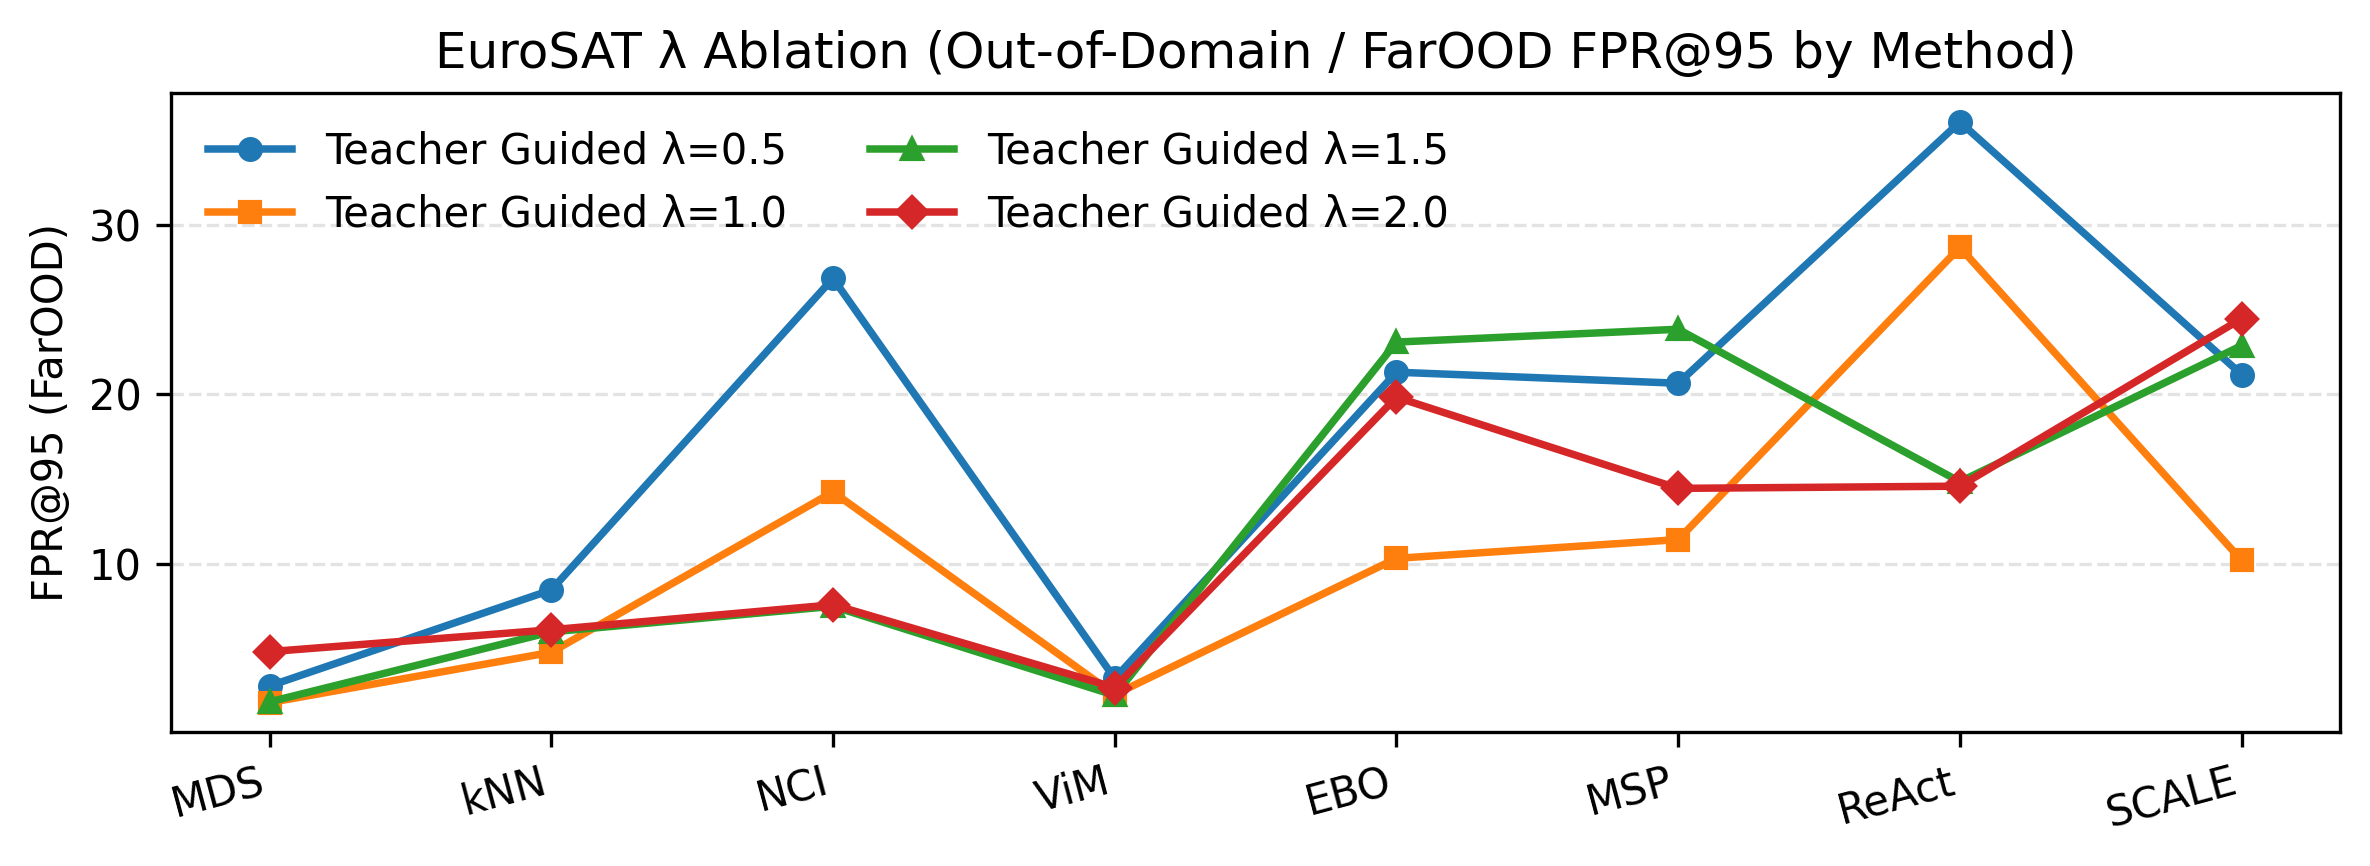
\includegraphics[width=0.88\textwidth,height=0.64\textheight,keepaspectratio]{dsc_eurosat_lambda_ablation.png}
\end{center}
\scopefooter{The effect is scorer-dependent; distance methods are comparatively stable near the default $\lambda_{\mathrm{TGT}}=1$.}
\end{frame}

\begin{frame}{Backup: Formal Hallucination Feasibility Argument}
\begin{enumerate}
  \item Residual computation makes later activations functions of earlier states and intervening transformations.
  \item A learned compressor obeys data processing:
  \begin{align*}
    I(f_\theta(H_i);f_\theta(H_j))\le I(H_i;H_j).
  \end{align*}
  \item InfoNCE lower-bounds view mutual information:
  \begin{align*}
    I(Z_i;Z_j)\ge \log K-\mathcal{L}_{\mathrm{InfoNCE}}.
  \end{align*}
  \item Loss below the no-information floor establishes positive learned-view dependence; downstream performance separately shows that the supervised slice is label relevant.
\end{enumerate}
\end{frame}

\begin{frame}{Backup: Hallucination Evaluation Grid}
\begin{itemize}
  \item \textbf{Models}: Llama-3.1-8B-Instruct and Qwen3-8B.
  \item \textbf{Datasets}: HotpotQA, Natural Questions, PopQA, SciQ, SearchQA.
  \item \textbf{Signal families}:
  \begin{itemize}
    \item Output-space scalar scores.
    \item Single-pass activation readers.
    \item Ten-sample uncertainty and consistency methods.
  \end{itemize}
  \item \textbf{Training}: a separate probe for each model--dataset cell; five seeds.
  \item \textbf{Metric}: AUROC against the automatic evaluator's correct/incorrect label.
\end{itemize}
\end{frame}

\begin{frame}{Backup: Hallucination-Study Scope}
\begin{itemize}
  \item \textbf{White-box requirement}: the detector needs intermediate activations.
  \item \textbf{Operational label}: incorrect short answers under an automatic evaluator are treated as hallucinations.
  \item \textbf{Model scope}: two open-weight 8B models; no closed API systems.
  \item \textbf{Task scope}: five short-answer QA datasets; no long-form, citation-grounded, or conversational generation.
  \item \textbf{Metrics not evaluated}: AUPRC, calibration error, and FPR@95.
  \item \textbf{Unresolved result}: ACT-ViT leads on Natural Questions for both models, and the cause is not yet isolated.
\end{itemize}
\end{frame}

\begin{frame}[allowframebreaks,noframenumbering]{References}
\footnotesize
\nocite{hendrycks2016baseline,huang2020survey,li2023halueval,lin2021truthfulqa,chen2020simple,selvaraju2017grad,oquab2023dinov2,Papyan2020nc,barshalom2025actvit,farquhar2024detecting,khosla2020supervised,oord2018representation}
\bibliography{references}
\end{frame}

\end{document}
